% !TEX root = thesis.tex
\chapter{Facebookの顔画像認識と深層学習技術}
この章では、Deep Learningを実際にWeb工学の問題に適用した例を挙げる。\par
ソーシャルメディアのユーザ属性を推定することは、マーケティングやネット広告の最適化において有益である。ここでは、公開プロフィールの一種であるプロフィール画像に着目する。入力となるプロフィール画像と、推定する目標であるユーザ属性のセットを用いて、Deep Learningを行わせることで、より精度の高いユーザ属性推定を目指す。

\section{背景}
ソーシャルメディアのユーザプロフィールから、そのユーザの属性を推定するためのアルゴリズムが求められている。\\
マーケティングや、ネット広告の最適化などに応用可能で、ビジネス面において大きな貢献が期待できる。\par
ユーザ属性の推定元としては、名前 / 日記 / ツイートなどのテキストデータ、プロフィールなどの画像、友達関係などが挙げられる。 \cite{pennacchiotti2011a-machine}\\

テキストデータは量が豊富だが、ソーシャルメディアの種類によっては、「友達のみ公開」などの設定がされている。ネット広告を載せる企業の視点から見ると、常に自由にアクセスできるとは限らない。\\

一方プロフィール画像は、ほぼ全てのソーシャルメディアにおいて、全員に公開されている。ネット広告企業からでも、必ずチェックできる。\\

画像からユーザ属性を推定できれば、より多くの場面で、効率の良いマーケティングが可能になる。これはテキストベースの方法にはない、大きなメリットである。\\

しかし、プロフィール画像を元データとした研究はまだメジャーではない。\\
最終的に、ソーシャルメディアのプロフィール画像が与えられれば、ユーザ属性を推定できる状態を目指す。\\
その過程として、今回の領域プロジェクトでは、「Facebook」より「プロフィール顔画像」に限定してのユーザ推定を試みる。\par

\begin{figure}[tbp]
 \begin{center}
  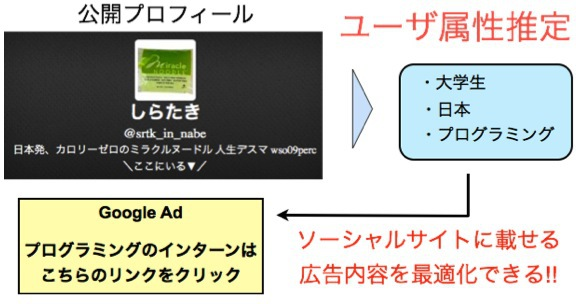
\includegraphics[width=100mm]{img/c6/prof2prop}
 \end{center}
 \caption{ユーザ属性推定の必要性}
 \label{c6_prof2prop}
\end{figure}

公開プロフィールからユーザ属性を推定するというアプローチによる過去の研究としては、Twitterのプロフィールやツイート内容、フォロー関係などから、ユーザ属性を割り出したものがある\\\cite{pennacchiotti2011a-machine}。この研究では、「スターバックスが好きか」「支持政党は民主党と共和党のどちらか」「どの民族 (ethnicity)に属しているか」といった情報を推定している。\\なお、この研究においては、プロフィール写真はユーザ属性を推定する参考になりにくいとされている。彼らに拠れば、ソーシャルメディアのユーザーは、必ずしもプロフィール画像にユー
ザ本人の画像を用いるわけではない。むしろ、有名人やキャラクターの画像、好きなブランドのロゴなど、あまり本人の属性推定に役立たないケースもある。図\ref{c6_pic_sample}

\begin{figure}[tbp]
 \begin{center}
  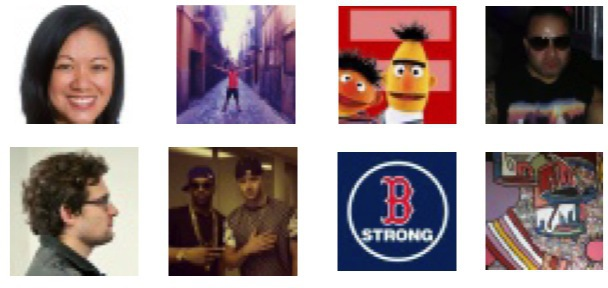
\includegraphics[width=100mm]{img/c6/pic_sample}
 \end{center}
 \caption{Facebookにおけるプロフィール画像の例}
 \label{c6_pic_sample}
\end{figure}

\section{問題設定}

\begin{figure}[tbp]
 \begin{center}
  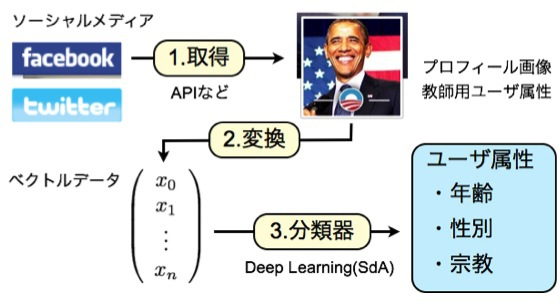
\includegraphics[width=100mm]{img/c6/concept}
 \end{center}
 \caption{提案手法}
 \label{c6_concept}
\end{figure}

\section{実験方法の詳細}

\begin{figure}[tbp]
 \begin{center}
  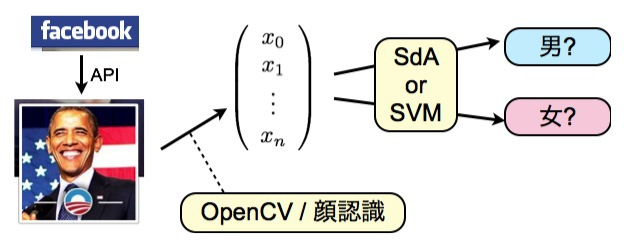
\includegraphics[width=80mm]{img/c6/expr}
 \end{center}
 \caption{今回の実験の模式図}
 \label{c6_expr}
\end{figure}

\begin{figure}[tbp]
 \begin{center}
  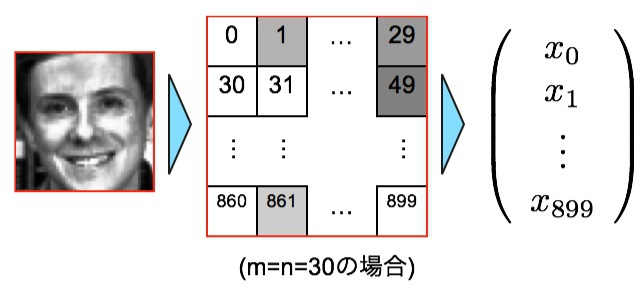
\includegraphics[width=80mm]{img/c6/conv}
 \end{center}
 \caption{画像から入力ベクトルへの変換方法}
 \label{c6_conv}
\end{figure}

\begin{figure}[tbp]
 \begin{center}
  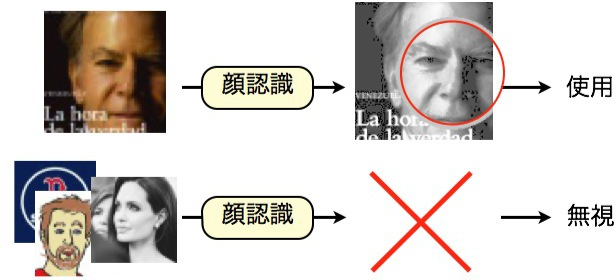
\includegraphics[width=80mm]{img/c6/pic_judge}
 \end{center}
 \caption{プロフィール画像からの顔画像抽出方法}
 \label{c6_pic_judge}
\end{figure}

\section{結果}

\begin{figure}[tbp]
 \begin{center}
  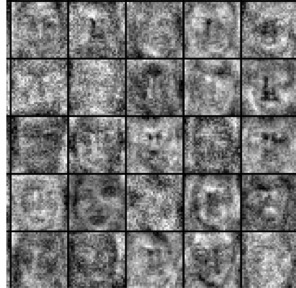
\includegraphics[width=100mm]{img/c6/filter}
 \end{center}
 \caption{実験で学習されたフィルター}
 \label{c6_filter}
\end{figure}